\section{Ricapitolazione di quanto visto finora}
\begin{description}
    \item[Modello relazionale]
    \item[Concetto relazione come variazione] (attributi, campi) di relazione matematica (tabella)
    \item[Schema e istanza:] $R(A_1, A_2, ..., A_n)$ per la relazione, $r(a_1, a_2, ..., a_n)$ per le istanze
    \item[Basi di dati come insieme di relazioni] $R = {(A_1, A_2, ..., A_n)}$
    \item[Superchiave:] insieme di attributi per cui la relazione R di cui è superchiave in cui non c'è nessuna tupla che si ripete. L'insieme di tutti gli attributi di una relazione è un esempio di superchiave.
    \item[Superchiave minimale (o CHIAVE):] quella che non contiene nessun'altra sottochiave, o nessun altro sottoinsieme di attributi.
    \item[Valore nullo:] "null", esiste per alcuni attributi, mentre altri non possono avere valore nullo; è un po' come facevamo in E-R, quando mettavamo cardinalità (0, 1) per un attributo in modo da indicarne l'opzionalità.
    \item[Vincoli di inter e intra relazionali:] vedremo oggi
    \item[Chiave Primaria:] vedremo oggi
\end{description}

\section{Tipi di vincoli}
\begin{description}
    \item[vincoli intrarelazionali:]
    \item vincoli su valori (o di dominio)
    \item vincoli di tupla
    \item vincoli di chiave (valuta le tuple nel complesso. es. non possono esistere due tuple con uno stesso valore per un particolare attributo A chiave).
    \item[vincoli interrelazionali] (coinvolge più relazioni): 
    \item vincoli di integrità referenziale
\end{description}
Tre concetti:
\begin{itemize}
    \item superchiave
    \item superchiave minimale (o Chiave)
    \item Chiave primaria
\end{itemize}
La \textbf{chiave primaria} non contiene attributi nulli. Sottoinsieme di attributi per cui è impossibile definire una superchiave minimale e per cui è impossibile avere attributi nulli.
\\Es.: tabella pag 65 universitari: la tabella avrà sempre una superchiave minimale, la matricola, che non può avere valore nullo (altrimenti come li identifichiamo gli studenti?) e questa è la \textbf{chiave primaria}.

\subsection{Importanza delle chiavi}
L'esistenza delle chiavi garantisce l'accessibilità a ciascun dato della base di dati.
\\Le chiavi permettono di correlare i dati in relazioni diverse: il modello relazionale è basato su valori.
\begin{center}
    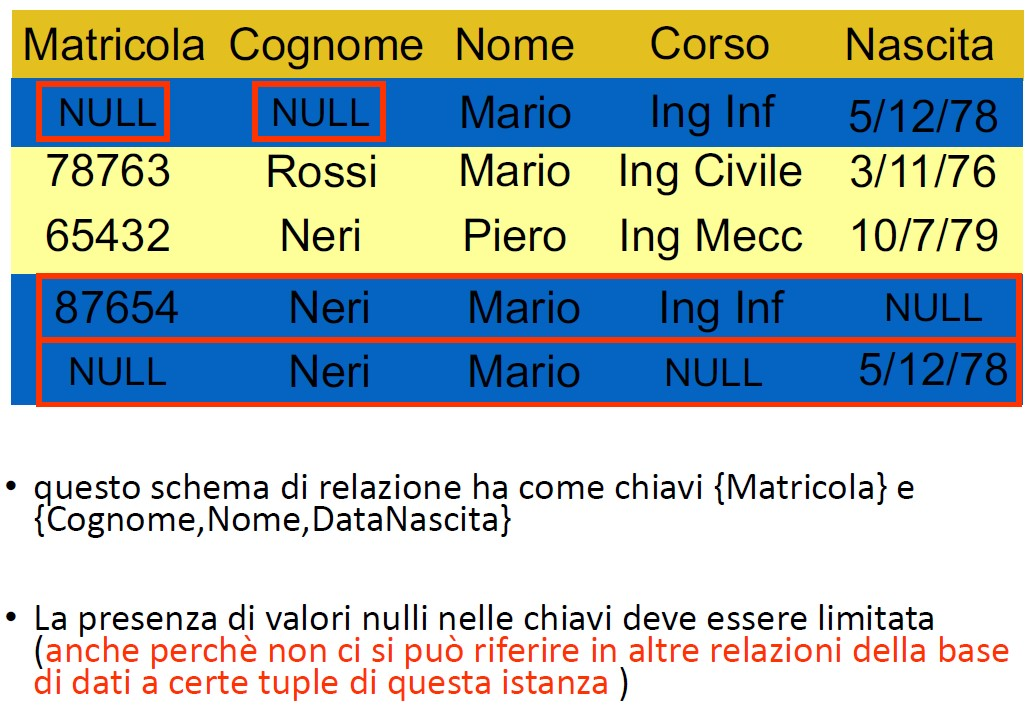
\includegraphics[width=0.5\textwidth]{img/MR_chiavi777.jpg}
\end{center}
La slide 71 mi riporta un esempio in cui i dati sono rappresentati in 3 tabelle scorrelate e relativamente indipendenti fra loro. Nella slide successiva viene mostrato l'output che avremmo se provassimo a rappresentare i dati in una sola tabella. Che non funzionerebbe tanto perché ci sarebbero troppe ripetizioni e poi avremmo anche molti valori nulli. Questa rappresentazione era da citare però perché mostra il comportamento di NoSQL.

\section{Vincolo di integrità referenziale}
Un \textbf{vincolo di integrità referenziale} (\textit{"foreign key"}) fra gli attributi $X$ di una relazione $R_1$ e un'altra relazione $R_2$ impone ai valori su $X$ in $R_1$ di comparire come valori della chiave primaria di $R_2$.
\\All'esame dovremo scegliere noi la chiave primaria (sottolineandola) e dire quali attributi vanno a formare il vincolo, ovvero a comporre la chiave primaria.
\begin{center}
    \includegraphics[width=0.5\textwidth]{img/MR_integrità_referenziale1.jpg}
\end{center}
\begin{center}
    \includegraphics[width=0.5\textwidth]{img/MR_integrità_referenziale2.jpg}
\end{center}
Leggi tu le slide, ora un esercizio di esempio.

\section{Esercizi di esempio}
\subsection{Es.: prestito di libri}
\begin{center}
    
\includegraphics[width=0.5\textwidth]{img/MR_es_prestitolibri1.jpg}
\end{center}
Quello che dobbiamo fare noi è scegliere la chiave primaria e dire quali attributi vanno a formare il vincolo, ovvero a comporre la chiave primaria.
\begin{center}
    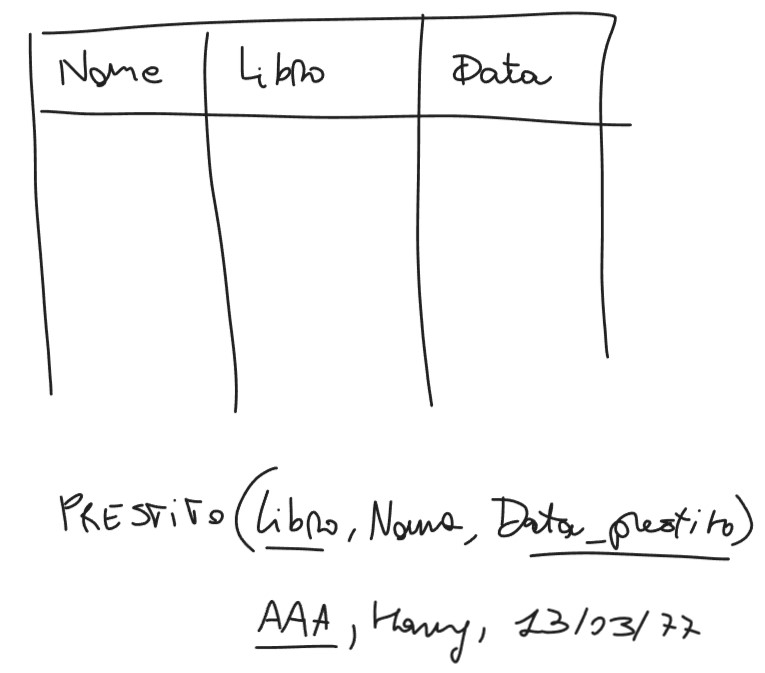
\includegraphics[width=0.5\textwidth]{img/MR_es_prestitolibri2.jpg}
\end{center}
\begin{center}
    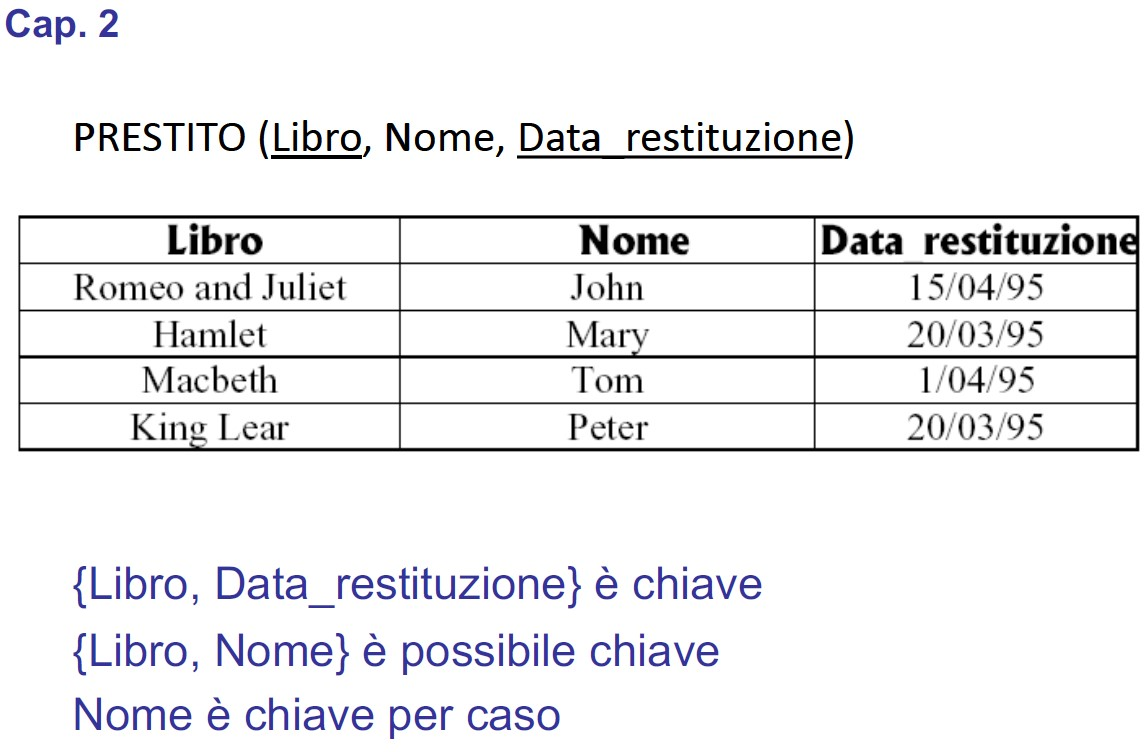
\includegraphics[width=0.5\textwidth]{img/MR_es_prestitolibri3.jpg} 
\end{center}

\subsection{Altro esempio}
Facciamo una sorta di reverse ingeniering: prendiamo una tabella e cerchiamo di capire come è stata fatta.
\\Ovvero: descrivere in linguaggio naturale le informazioni organizzate nella base di dati. 
Individuare: 
\begin{enumerate}
    \item le chiavi (primaria, e almeno 1 superchiave)
    \item i vincoli di integrità referenziale
    \item gli attributi su cui NON possono essere ammessi valori nulli.
\end{enumerate} 
Per il punto 1.:
\begin{center}
    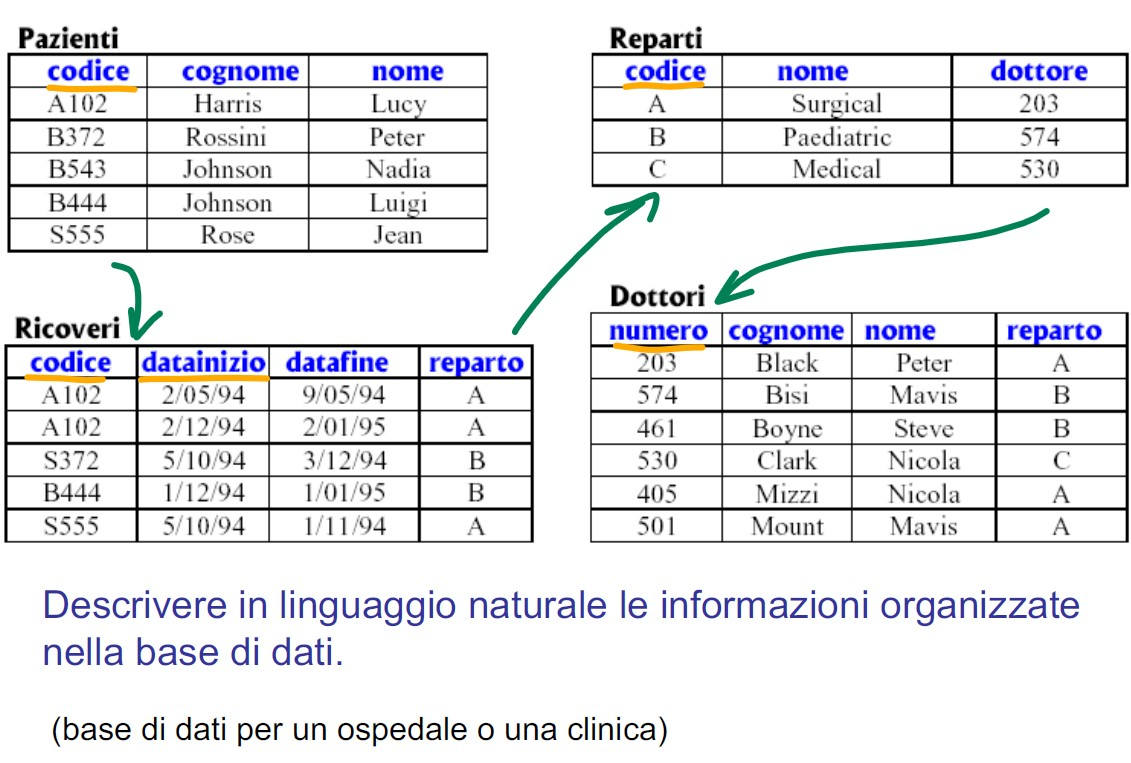
\includegraphics[width=0.5\textwidth]{img/MR_es_altro1.jpg}
\end{center}
Per il punto 2.: c'è un vincolo di integrità referenziale non rispettato (ovvero, non esiste nella tabella dei pazienti il paziente identificato dal codice S372 che è possibile vedere nella tabella dei ricoveri).
\\Per il punto 3.: tutte le chiavi primarie ovviamente.
\subsubsection{Soluzioni}
\begin{enumerate}
    \item I valori nulli sono permessi solo negli attributi che non sono
chiave primaria.
Alcuni non hanno molto senso (nome cognome in Dottori)
Codice per la relazione PAZIENTI
{Paziente, datainizio}, {Paziente, datafine} per la relazione RICOVERI (si
assume che un paziente sia ricoverato –dimesso- una sola volta in un
giorno)
Numero per la relazione DOTTORI
Codice per la relazione REPARTI
\item
I vincoli referenziali sono fra:
• Codice in RICOVERI e Codice in PAZIENTI
•Reparto in RICOVERI e Codice in REPARTI
• Dottore in REPARTO e Numero in DOTTORI
• Reparto in DOTTORI e Codice in REPARTI
    \item I valori nulli sono permessi solo negli attributi che non sono chiave primaria. Alcuni non hanno molto senso (nome cognome in Dottori)
\end{enumerate}

\subsection{Altro esempio: stazione}
\begin{center}
    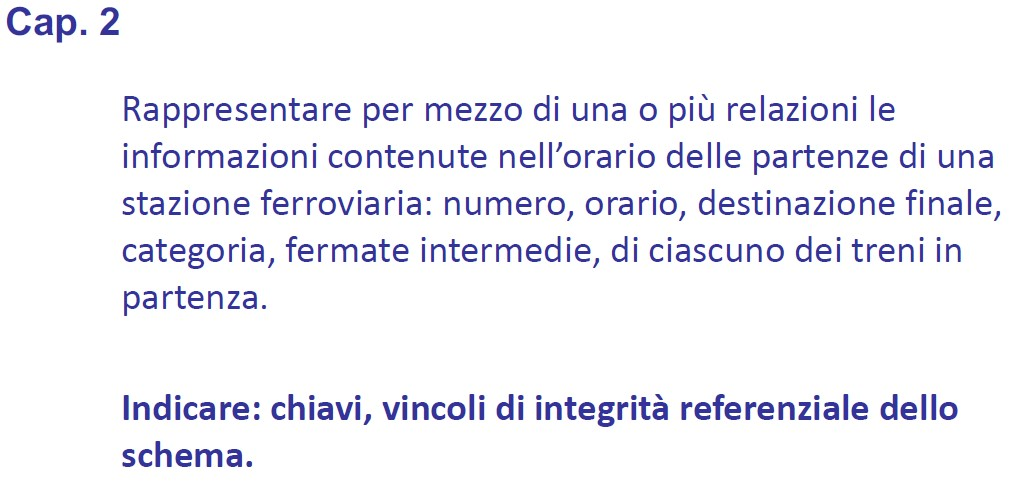
\includegraphics[width=0.5\textwidth]{img/MR_es_stazione1.jpg}
\end{center}
Sol. aula:
\begin{verbatim}
    TRENO (Tipo, \underline{Numero}, DestinazioneFinale, OrarioPartenza)
\end{verbatim}
                            \uparrow
\begin{verbatim}
    FERMATE (\underline{Nome, Numero,} Orario)
\end{verbatim}
Sol. slides:
\begin{verbatim}
    PARTENZE (\underline{Numero}, OrarioPartenza, Destinazione Finale, Categoria)
    FERMATE (\underline{Treno, Stazione}, Orario)
\end{verbatim}
La prima relazione rappresenta tutti i treni in partenza dalla stazione ferroviaria, distinti per il Numero (chiave primaria della relazione).
\\La seconda rappresenta le fermate intermedie per ciascun treno in ciascuna stazione (chiave primaria composta da Treno e Stazione) con vincolo referenziale fra Treno in STOP e Numero in PARTENZE.
\\Manca qualcosa: relazione treno.
\begin{verbatim}
    TRENO(\underline{Numero}, Categoria)
\end{verbatim}
La terza rappresenta le fermate intermedie per ciascun treno in ciascuna stazione (chiave primaria composta da Treno, Stazione e orario).

\subsection{Altro esempio: azienda}
\begin{center}
    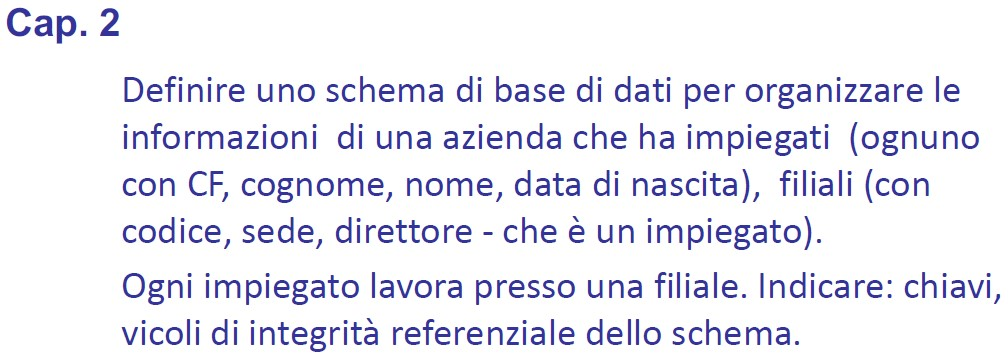
\includegraphics[width=0.5\textwidth]{img/MR_es_azienda1.jpg}
\end{center}
Quante relazioni ci servono? 2. Ogni filiale ha più impiegati. Quindi una tabella per filiali, una per impiegati, una per azienda.
\begin{verbatim}
    IMPIEGATO (\underline{CF}, Nome, Cognome, Nascita, Filiale)
    FILIALE (\underline{Codice}, Sede, Direttore)
\end{verbatim}
Ellisse con freccia da IMPIEGATO(..., Filiale) a FILIALE(Codice, ...) per indicare il vincolo di integrità referenziale.
\\Ellisse con freccia da FILIALE(..., Direttore) a IMPIEGATO per indicare il vincolo di integrità referenziale.

\subsection{Altro esempio: radio}
\begin{center}
    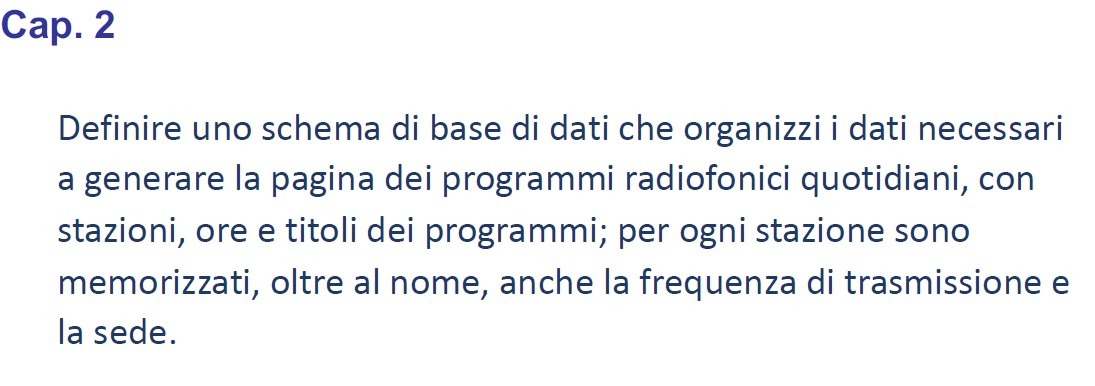
\includegraphics[width=0.5\textwidth]{img/MR_es_radio1.jpg}
\end{center}
Quante relazioni ci servono? 2.
\begin{verbatim}
    PROGRAMMI (\underline{Titolo, Stazione}, Orario) 
    STAZIONE (\underline{Nome}, Frequenza, Sede)
\end{verbatim}
Magari all'interno di PROGRAMMI(...) basta da solo il Titolo per identificare univocamente un programma all'interno di una stazione.
\begin{center}
    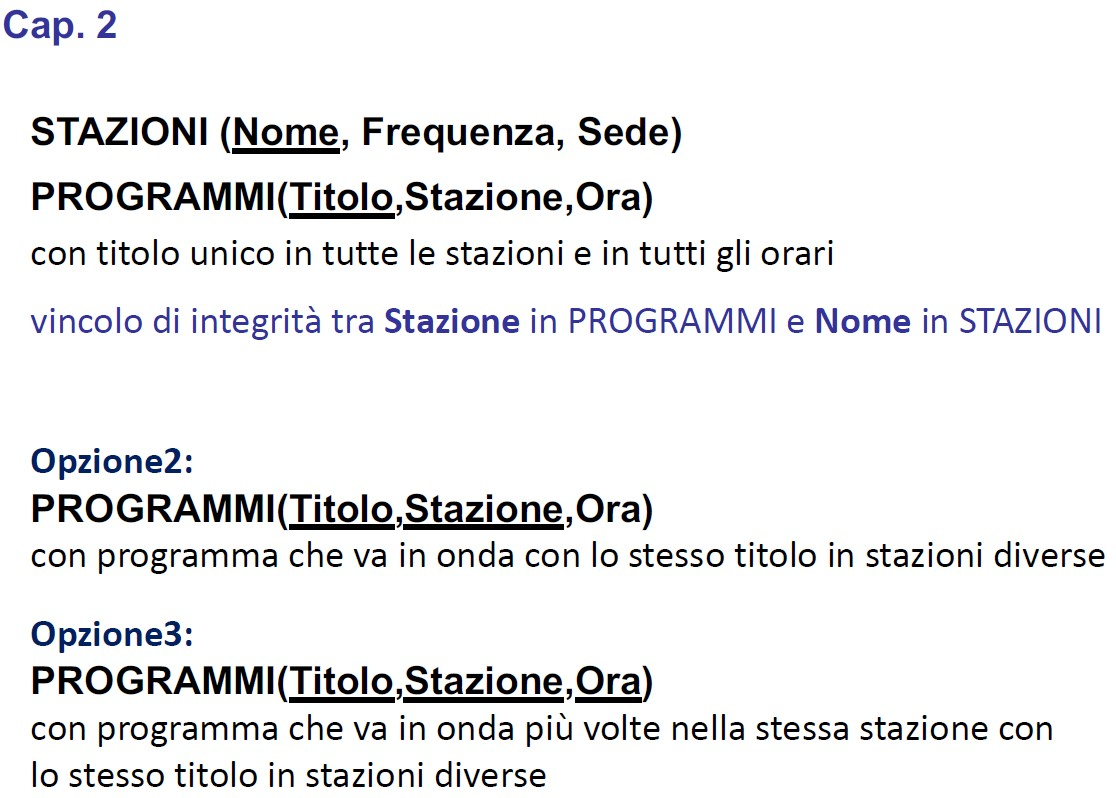
\includegraphics[width=0.5\textwidth]{img/MR_es_radio2.jpg}
\end{center}

\section{Esempio di esercizio MR che troveremo all'esame}
\begin{center}
    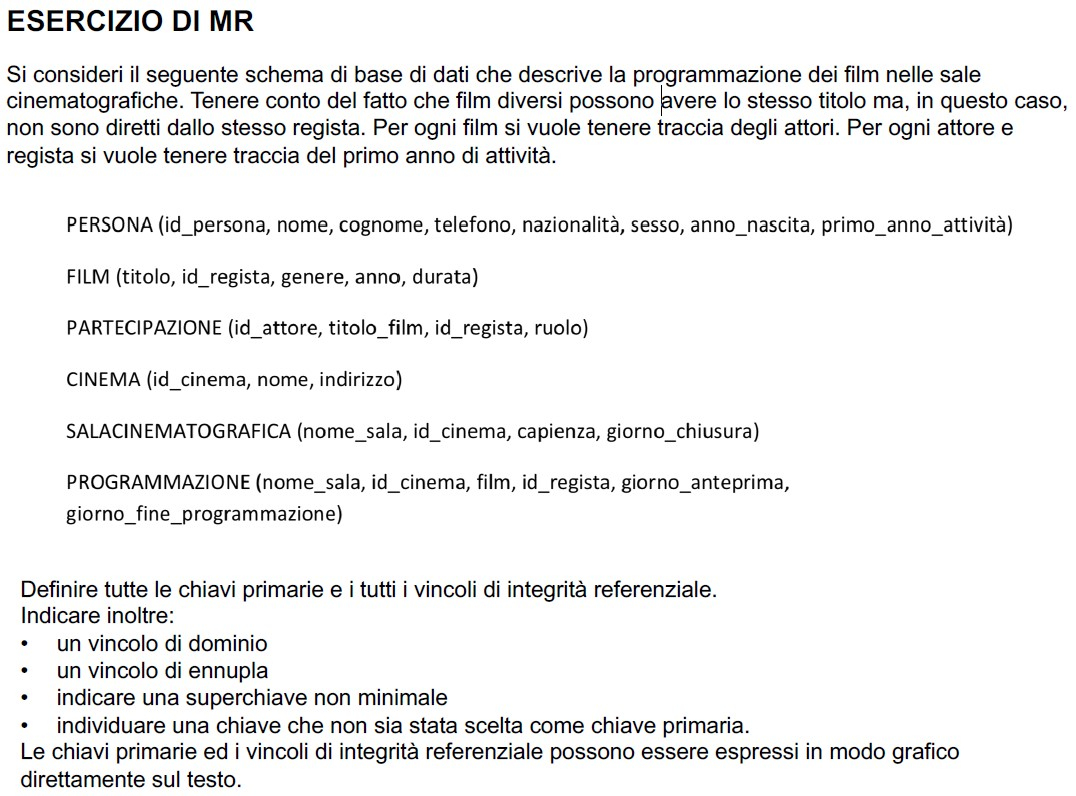
\includegraphics[width=0.5\textwidth]{img/MR_facsimile_esame1.jpg}
\end{center}
\begin{center}
    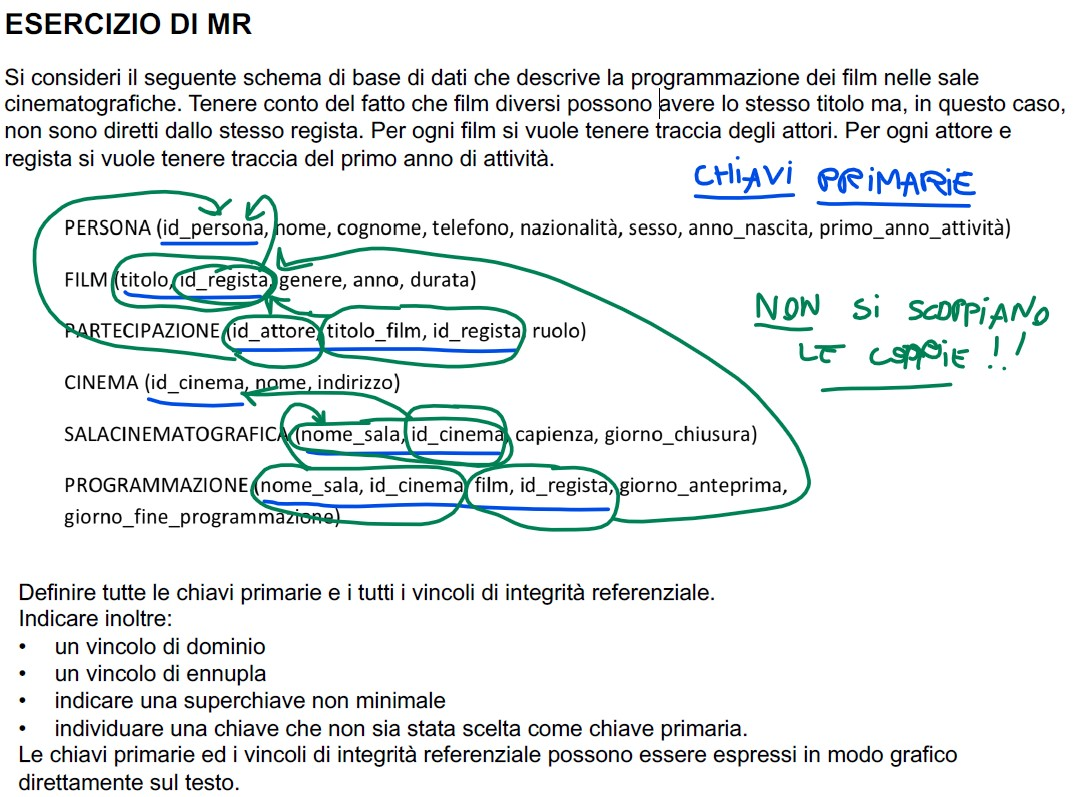
\includegraphics[width=0.5\textwidth]{img/MR_facsimile_esame2.jpg}
\end{center}
\begin{center}
    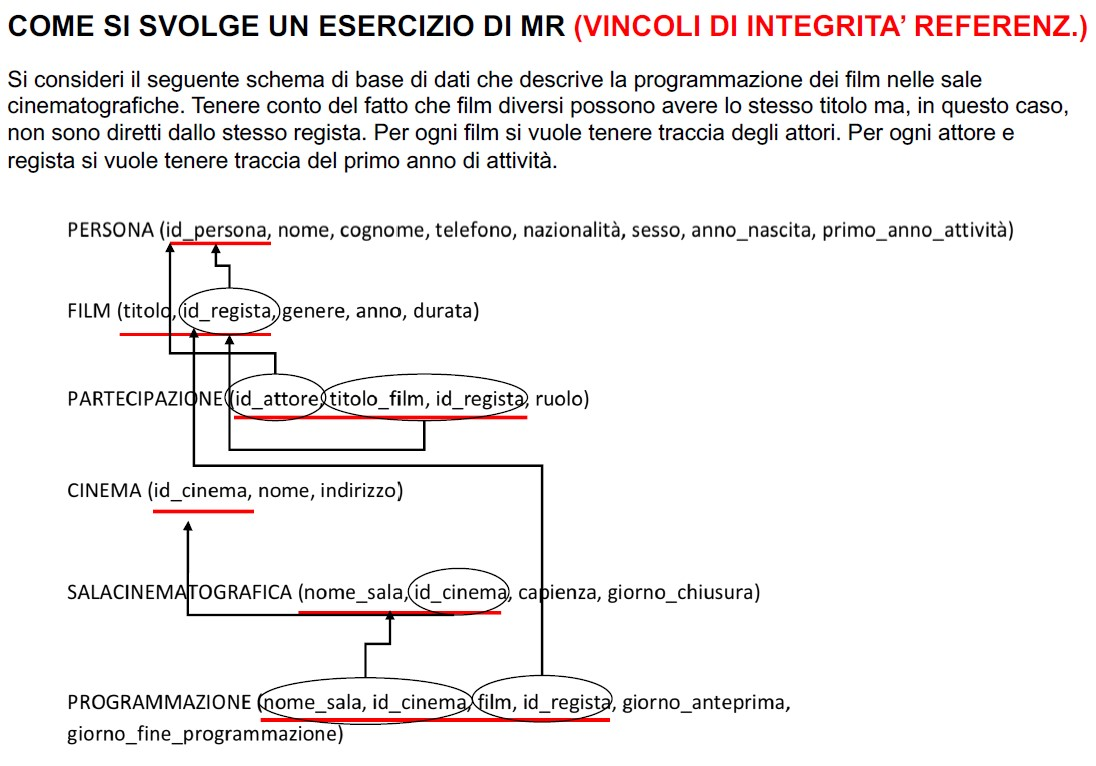
\includegraphics[width=0.5\textwidth]{img/MR_facsimile_esame3.jpg}
\end{center}


